\section{Method}

\begin{frame}
	\frametitle{Contributions}
	
	\Large
	
	\vspace{0.8cm}
	
	We present an automated approach for classifying Alzheimer's disease patients from MRI brain scans.
	
	\begin{enumerate}
		\item key points extracted with a \textbf{recent} feature extraction technique, called ORB
			  \cite{Rublee11}
		\item final set of features obtained by \textbf{defining} two \textbf{new} metrics:
			  \textbf{spatial position} of extracted key points and \textbf{their distribution} around
			  the patient's brain
		\item \textbf{fast} and \textbf{reliable} approach for a straightforward deploy in clinical
			  applications
	\end{enumerate}
	
	\vspace{0.6cm}
	
	\tiny
	
	\cite{Rublee11} E. Rublee \emph{et al.}, ``ORB: an efficient alternative to SIFT or SURF'',
	International Conference on Computer Vision, 2011
\end{frame}

\begin{frame}
	\frametitle{Methodology}
	
	\Large
	
	\vspace{0.7cm}
	
	We focus on extracting features which are \textbf{key points} found in the image. In particular, we
	choose as features a set of key points from the MRI scan \textbf{computed} with the ORB feature
	extractor, and we \textbf{associate} to them their \textbf{spatial position} and
	\textbf{distribution} around the patient's brain.
	
	\begin{center}
		\begin{tikzpicture}
			\node at (-5.5,0) [draw=white,ultra thick,inner sep=0pt]
			{
				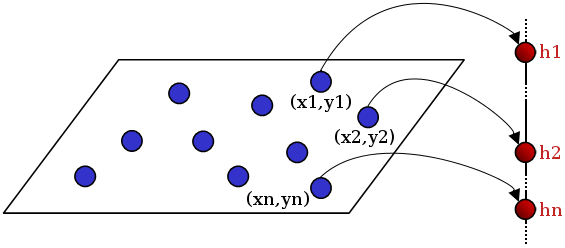
\includegraphics[height=2.5cm]{Figures/CantorHash}
			};
			\node at (0,0) [draw=white,ultra thick,inner sep=0pt]
			{
				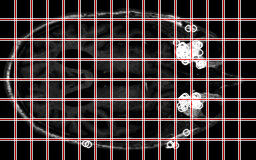
\includegraphics[height=2.5cm]{Figures/Histograms}
			};
		\end{tikzpicture}
	\end{center}
\end{frame}

\begin{frame}
	\frametitle{Methodology}
	\framesubtitle{Key point features}
	
	\Large
	
	\vspace{0.7cm}
	
	Many different approaches have been proposed for feature extraction. We focus on a
	\textbf{computationally-efficient} technique - called ORB - which is based on a FAST key point
	detector. It provides \textbf{good matching}, \textbf{slighlty} affected by image noise and
	\textbf{real-time} performance.
	
	\vspace{0.1cm}
	
	\begin{center}
		\begin{tikzpicture}
			\node at (-2.6,0) [draw=red,ultra thick,inner sep=0pt]
			{
				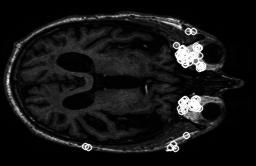
\includegraphics[height=2.5cm]{Figures/OrbKeypoint}
			};
			\node at (0,0) [draw=red,ultra thick,inner sep=0pt]
			{
				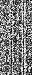
\includegraphics[height=2.5cm]{Figures/OrbDescriptor}
			};
		\end{tikzpicture}
	\end{center}
\end{frame}

\begin{frame}
	\frametitle{Methodology}
	\framesubtitle{Key point features}
	
	\Large
	
	\begin{columns}[T]
		\column{0.35\textwidth}
		
		\begin{center}
			\begin{tikzpicture}
				\node at (0,0) [draw=red,ultra thick,inner sep=0pt]
				{
					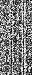
\includegraphics[height=3.5cm]{Figures/OrbDescriptor}
				};
			\end{tikzpicture}
		\end{center}
		
		\column{0.58\textwidth}
		
		\vspace{0.65cm}
		
		The feature descriptor of each key point is a \textbf{32-vector} of the pixel
		\textbf{intensity}. The image is described by a $ k \times 32 $ matrix, where $ k $ represents
		the number of key points found in the image.
		
		\column{0.05\textwidth}
	\end{columns}
\end{frame}

\begin{frame}
	\frametitle{Methodology}
	\framesubtitle{Feature extraction}
	
	\Large
	
	\vspace{0.4cm}
	
	We investigate different strategies for building the feature matrix based on the key points
	extracted from the MRI scans and their properties:
	
	\begin{enumerate}
		\item Image descriptor
		\item Histograms
		\item Cantor hash
		\item Histograms and Cantor hash
	\end{enumerate}
\end{frame}

\begin{frame}
	\frametitle{Methodology}
	\framesubtitle{Image descriptor}
	
	\Large
	
	\vspace{0.5cm}
	
	The image descriptor is built by \textbf{straightforwardly} considering the $ k \times 32 $ matrix
	representing the ORB descriptors associated to $ k $ key points of a MRI scan. Each element of the
	matrix is an integer within $ [0,255] $
	
	\begin{center}
		\begin{tikzpicture}
			\node at (0,0) [draw=red,ultra thick,inner sep=0pt]
			{
				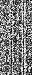
\includegraphics[height=3.1cm]{Figures/OrbDescriptor}
			};
		\end{tikzpicture}
	\end{center}
\end{frame}

\begin{frame}
	\frametitle{Methodology}
	\framesubtitle{Histograms}
	
	\Large
	
	\vspace{0.3cm}
	
	Key points \textbf{spatial distribution} is obtained by:
	
	\vspace{-0.1cm}
	
	\begin{itemize}
		\item \textbf{dividing} the MRI scan in a grid $ G = r \times c $ 
		\item for each cell of the grid we compute a \textbf{histogram} representing the number of key
			  points belonging to such a cell
	\end{itemize}
	
	In this way, we build a feature vector by providing the number of key points belonging to every
	cell of the grid. The histogram value for each cell is bounded between $ [0,k] $ and the $
	\sum_{i=1}^r \sum_{j=1}^c G(i,j) = k $
\end{frame}

\begin{frame}
	\frametitle{Methodology}
	\framesubtitle{Cantor hash}
	
	\Large
	
	\vspace{0.3cm}
	
	Key points \textbf{spatial position} is obtained by computing the \emph{Cantor} hash for each key
	point in order to \textbf{map} its Cartesian position into a mono-dimensional space.
	
	\vspace{0.2cm}
	
	In this case, the feature vector contains the hash value $ h(x,y) $ of all key points. The
	Cartesian coordinates $ x $ and $ y $ are both 8-bit since they represent grey-scale pixel
	
	\begin{center}
		\begin{tikzpicture}
			\node at (0,0) [draw=white,ultra thick,inner sep=0pt]
			{
				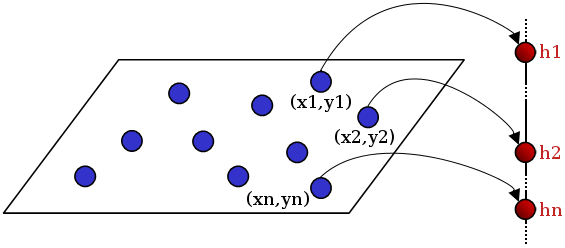
\includegraphics[height=2.5cm]{Figures/CantorHash}
			};
		\end{tikzpicture}
	\end{center}
\end{frame}

\begin{frame}
	\frametitle{Methodology}
	\framesubtitle{Histograms and Cantor hash}
	
	\Large
	
	\vspace{0.3cm}
	
	We decide to use also the \textbf{combination} of histograms and Cantor hashing for building the
	feature matrix considering \textbf{at the same time} the spatial position of key points as well as
	their distribution around the patient brain.
	
	\vspace{0.3cm}
	
	The Cantor hashing function provides information on the \textbf{exact position} of each key point
	in the brain whilst in the histogram, we use the position of the key points to approximate the
	\textbf{geometrical shape} of them around the brain
\end{frame}

\begin{frame}
	\frametitle{Methodology}
	\framesubtitle{Feature matrix}
	
	\Large
	
	\vspace{0.3cm}
	
	We collect $ n $ brain patients' scan, each one with its $ m $ features and their class label
	(e.g., AD, MCI, LMCI, CN). Every patient's scan $ i \in [1,n] $ with its $j \in [1,m] $ features is
	represented by the vector
	
	\vspace{-0.5cm}
	
	\begin{equation*}
		f_i =(f_{i1}, f_{i2}, \cdots, f_{ij}, \cdots, f_{im}, f_{ic}) \;\;\;\;\;\; 
	\end{equation*}

	where $ f_{ij} \in \mathbb{Z} $ and $ f_{ic} \in {\{AD, MCI, LMCI, CN\}} $.
	
	\vspace{0.3cm}
	
	The \textbf{data matrix} is obtained by the \textbf{union of vectors} $ f_1, f_2, \cdots, f_n $,
	where rows represent the MRI patients' scan and columns the features
\end{frame}

\begin{frame}
	\frametitle{Methodology}
	\framesubtitle{Classification}
	
	\Large
	
	\vspace{0.3cm}
	
	We use Support Vector Machines (SVMs) which is a very \textbf{successful} approach for classifying
	data especially in \textbf{high dimensional} feature spaces.
	
	\vspace{0.3cm}
	
	We choose SVMs, because of their \textbf{proven success} in imaging classification and their
	\textbf{good generalisation ability}. This property is obtained by maximising the margin between
	the closest points to the hyperplane (called support vectors) and the hyperplane defining the
	boundaries of different classes
\end{frame}
